\documentclass[border=3pt,tikz]{standalone}
% Shared look for every TikZ figure in these notes.
% Included by each standalone figure file; also keeps the figures consistent
% with the colours used in the PDF and on the website.

\usepackage{tikz}
\usepackage{pgfplots}
\pgfplotsset{compat=1.18}
\usetikzlibrary{arrows.meta, decorations.markings, decorations.pathmorphing,
                patterns, calc, positioning}
\usepackage{amsmath}

% Series colours are the three validated categorical slots also used by the
% interactive widgets, so a path drawn in the printed notes and the same path on
% the website are the same colour. They clear the colour-vision-deficiency and
% contrast checks as a set; every path is direct-labelled as well, so colour is
% never the only thing carrying identity.
\definecolor{duPurple}{HTML}{68246D}
\definecolor{duBlue}{HTML}{2A78D6}
\definecolor{duRed}{HTML}{EB6834}
\definecolor{duGreen}{HTML}{1BAF7A}
\definecolor{duGrey}{HTML}{4D4D4D}

\tikzset{
  % heavier default lines and arrow tips, so diagrams stay clear when zoomed
  every picture/.append style = {line width=0.7pt, >={Stealth[length=3mm]}},
  axisline/.style   = {-{Stealth[length=3.4mm]}, line width=1.0pt, black},
  path1/.style      = {duBlue,   line width=1.6pt},
  path2/.style      = {duRed,    line width=1.6pt},
  path3/.style      = {duGreen,  line width=1.6pt},
  statedot/.style   = {circle, fill=black, inner sep=1.8pt},
  arrowhead/.style  = {decoration={markings,
                        mark=at position #1 with {\arrow{Stealth[length=3.4mm]}}},
                       postaction={decorate}},
  lbl/.style        = {font=\normalsize},
  slbl/.style       = {font=\small, duGrey},
  workfill/.style   = {duPurple, opacity=0.16},
}

% larger labels in plots as well
\pgfplotsset{every axis/.append style={label style={font=\normalsize}, tick label style={font=\small}, line width=0.9pt}}

% Barometer: an inverted tube in a bath of liquid. A is on the free surface of
% the bath (open to the atmosphere); B is inside the tube at the same level.
\begin{document}
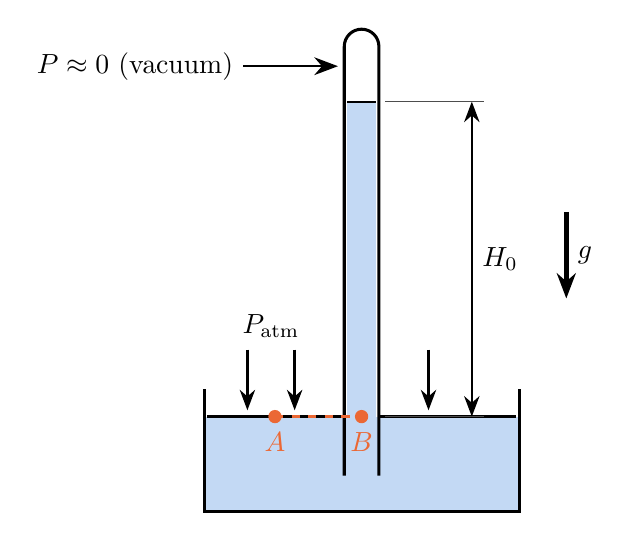
\begin{tikzpicture}[x=1cm, y=1cm]
  \colorlet{liq}{duBlue!28}
  % ---- bath --------------------------------------------------------------
  \fill[liq] (-2.0,0) rectangle (2.0,-1.2);
  \draw[line width=1.1pt] (-2.0,0.35) -- (-2.0,-1.2) -- (2.0,-1.2) -- (2.0,0.35);
  % ---- tube: liquid column, then (near) vacuum at the top ----------------
  \fill[liq] (-0.18,-0.75) rectangle (0.18,4.0);
  \fill[white] (-0.18,4.0) rectangle (0.18,4.7);
  \draw[line width=1.1pt] (-0.22,-0.75) -- (-0.22,4.7) arc[start angle=180, end angle=0, radius=0.22] -- (0.22,-0.75);
  \draw[line width=0.8pt] (-0.18,4.0) -- (0.18,4.0);
  % free surface of the bath (drawn over the tube walls only outside)
  \draw[line width=0.8pt] (-1.96,0) -- (-0.22,0);
  \draw[line width=0.8pt] (0.22,0) -- (1.96,0);
  % ---- labels at the top -------------------------------------------------
  \draw[-{Stealth[length=3mm]}, line width=0.9pt] (-1.5,4.45) -- (-0.3,4.45)
    node[pos=0, left, font=\normalsize] {$P \approx 0$ (vacuum)};
  % ---- atmospheric pressure on the free surface -------------------------
  \foreach \x in {-1.45,-0.85, 0.85} {
    \draw[-{Stealth[length=2.6mm]}, line width=0.9pt] (\x,0.85) -- (\x,0.08);
  }
  \node[font=\normalsize] at (-1.15,1.15) {$P_\text{atm}$};
  % ---- column height H0 --------------------------------------------------
  \draw[duGrey, line width=0.6pt] (0.3,4.0) -- (1.55,4.0);
  \draw[duGrey, line width=0.6pt] (0.3,0) -- (1.55,0.0);
  \draw[{Stealth[length=2.6mm]}-{Stealth[length=2.6mm]}, line width=0.9pt] (1.4,0) -- (1.4,4.0)
    node[midway, right, font=\normalsize] {$H_0$};
  % ---- gravity -----------------------------------------------------------
  \draw[-{Stealth[length=3.2mm]}, line width=1.6pt] (2.6,2.6) -- (2.6,1.5)
    node[midway, right, font=\normalsize] {$g$};
  % ---- points A and B at the same level ---------------------------------
  \draw[duRed, dashed, line width=1pt] (-1.1,0) -- (0,0);
  \fill[duRed] (-1.1,0) circle (2.4pt) node[below=2pt, font=\normalsize\bfseries, text=duRed] {$A$};
  \fill[duRed] (0,0) circle (2.4pt);
  \node[font=\normalsize\bfseries, text=duRed, below=2pt] at (0,0) {$B$};
\end{tikzpicture}
\end{document}
